\chapter{Introduction}


% ***
% plan

% intro - general trend towards computer model so no animal/human cruelty or tests
% comp power not yet there
% tailored medicine
% mc method powerful techniques

% move onto mc methods
% history
% what are they
% examples
% applications

% thesis outline
% signpost chapters

% ***
The advent of the computer in the last 80 years has been a boon for society.
Increasing computing power is easily available, allowing higher-quality research, and research into topics once thought beyond human computation.
One topic where computers have revolutionised is medicine.
Computers have enabled advances in many areas including drug discovery~\cite{aaqvist1994new,lill2011computer}, patient diagnoses~\cite{liu2014early,sun2016computer}, and better imaging modalities~\cite{brooks1976principles,al2012digital}.
One particular area of focus where computers are or will be heavily used is personalised medicine.

Personalised medicine is where instead of a patient being treated with what works on an ``average'' patient, the treatment is tailored specifically for the patient.
This entails having fine grained knowledge of the patient down to the genome, to understand how various drug or treatments will affect the patient.
One particular area of research  in personalised medicine is into the so called ``digital twin''.
A digital twin as defined by A. El Saddik~\cite{el2018digital}:

\medskip
``A digital twin is a digital replica of a living or non-living physical entity.''
\medskip

\noindent Digital twins are currently heavily used in engineering to predict when various machinery will need to undergo maintenance.
The way the digital twin is used is that the machine has various sensors that feed data into a digital model of the machine, allowing predictions of how the machine will operate in its current condition.
Companies like Phillips use this in their MRI machines to help schedule downtime, and predict which parts the engineer will need on site, both of which minimises the downtime of the machine which is import for the hospital/clinic~\cite{henkvanhouten2018}.
At the heart of the digital twin method, is the ability to accurately model the object or living thing being studied.
This can be straightforward when the twin in question is a machine, as sensors can usually be attached to the various components to get feed back on the machines operation.
Machines also have the bonus of (normally) be completely understood so that modelling them is usually easy.
However, this is not as straightforward when dealing with biology.
First, we still do not have a complete understanding of the biology within humans.
Therefore, modelling a human accurately is not possible as various assumptions and approximations have to be made.
Second, to get accurate information on what is happening inside a patient, either ionising radiation needs to be used, or cameras inserted into the patient.
Both of these cannot be done for indefinite periods without causing harm or discomfort to the patient.
Therefore, continuous information on the inner functions of the body is not possible.
One area where information is more readily available is the skin.
Information on the skin function or dysfunction is normally diagnosed with light.
Light is also used in various treatments such as photodynamic therapy and tissue ablation, over various internal and external sites on the body.
Lights interaction over the whole spectrum, from the UV to the infrared, is readily modelled with techniques such as \gls*{mcrt}.
\Gls*{mcrt} allows a digital twin model of individual patient skin to be simulated.
This can then be used to tailor treatment regimes for the individual patient, or to predict treatment outcomes for specific patients.
The use of simulations techniques like \gls*{mcrt} allow testing \textit{in-silico}, which can negate the need to test on humans or animals.

\medskip
This thesis concerns the development of various \gls*{mcrt} models to help diagnose, optimise treatments and help predict which imaging modalities may be better.

% allow tests on digital couterpart, no need for invasive, painful or tests that may have adverse affects.
% Saves from animal testing too.
% used in industry -> example philips mri machine. used to keep track of equipment, id maintenance before they arise etc
% originally comes from industry
% parley this into humans, and thus mcrt
% personalised medicine 
% speak about mcrt a wee bit
% then link onto next paragraph

\section{Monte Carlo Method}\label{sec:mcmethod}
The Monte Carlo method is a numerical analysis technique based upon random numbers, which are used to calculate unknown variables in problems~\cite{cashwell1959practical,rogers1990monte}. 

The earliest use of the method is in Buffon's needle experiment of the 18$^{th}$ century~\cite{badger1994lazzarini,beckmann2015history,buffon1785histoire}. Buffon asked the question;

\medskip

``Suppose we have a floor made of parallel strips of wood, each the same width, and we drop a needle onto the floor. What is the probability that the needle will lie across a line between two strips?''

\medskip

The solution to this question is:
for a needle length \textit{l}, strip separation \textit{s}, where \textit{x} is the distance from the needle to the closest line, and $\theta$ is the angle of the needle with respect to the wood strips. Then using a simple geometrical argument, a needle crosses a strip if $x \leq \tfrac{l}{2} sin \theta$.

$x$ is distributed uniformly in [0, $\tfrac{s}{2}$], and $\theta$ in [0, $\tfrac{\pi}{2}$]. Therefore the probability density function for $x$ is $p(x)=\tfrac{2}{s}$, and $\theta$ is $p(\theta) = \tfrac{2}{\pi}$. The \gls*{pdf}, is a function of a variable that gives probability for a variable to a take a given value. The \gls*{pdf} is normalised over the whole range of the variable, in this case $x$, and $\theta$.
Thus, as $x$ and $\theta$ are independent variables, giving a joint probability of $p(x,\theta) = \tfrac{4}{s \pi}$.
So the probability of a needle of length $l$ ($l<s$) is:

\begin{equation}
P=\int_0^{\frac{\pi}{2}}\int_0^{\frac{l}{2}sin\theta}\frac{4}{s\pi}\ dx\ d\theta = \frac{2 l}{s \pi}\label{eqn:buffon}
\end{equation}


\Cref{eqn:buffon} can be used to carry out a Monte Carlo estimation of $\pi$. A simple rearrangement yields: $\pi = \tfrac{2l}{sP}$ where P is the ratio of needles crossing the line to the total number dropped. Laplace was the first to suggest that Buffon's needle experiment could be used to estimate $\pi$~\cite{beckmann2015history}. 
\Cref{fig:buffon-needle} shows an example of a simulation of Buffon's needle experiment.

\begin{figure}[!htb]
\centering
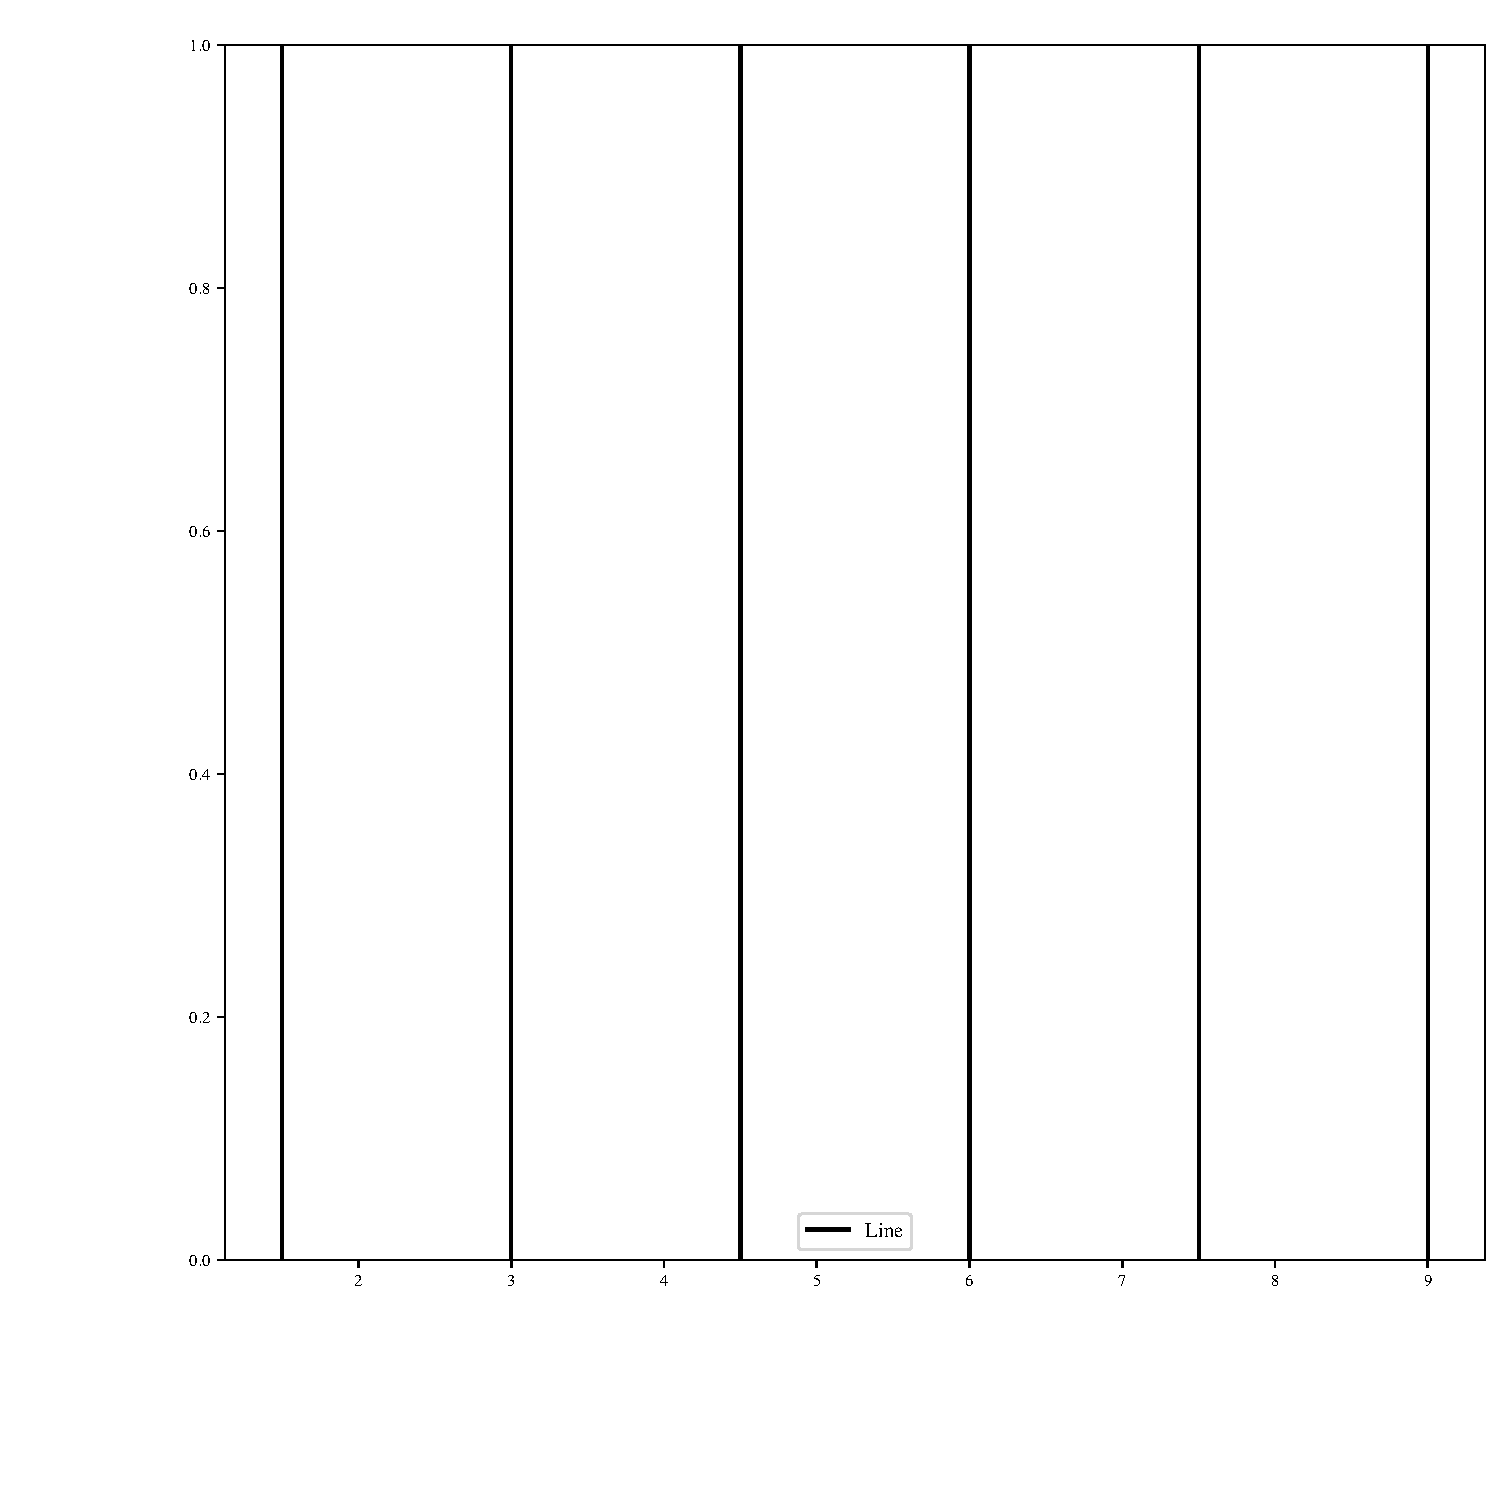
\includegraphics[width=.5\textwidth]{buffon.pdf}
\caption{Sample Buffon needle experiment. 100 needles are dropped on a 10 $\times$ 10 cm area with lines spaced 1.5~cm apart. If a needle lands on a line it is recorded and coloured blue, else it is red. This simulation gave a value of $\pi$ $\approx$ 3.10.}
\label{fig:buffon-needle}
\end{figure}

There are various different approaches to using the Monte Carlo method to obtain randomly sampled variables.
One analytical way of achieving this is the inverted sampling method.
The inverted sampling method can be summarised by the following steps for drawing a sample $X_i$ from an arbitrary PDF $p(x)$:

\medskip

1. Compute the \gls*{cdf} $P(x)=\int^{x}_{0}p(x')dx'$

2. Compute the inverse $P^{-1}(x)$

3. Obtain a uniformly distributed random number $\xi$

4. Finally, compute $X_i = P^{-1}(\xi)$

\medskip

If a given problem cannot use the inverted sampling method, as it may not be possible to get a PDF or analytically invert the CDF, then the rejection method can be used.
The rejection method is essentially a dart throwing method.
This means that points are drawn and compared to the function.
If the point lies under the function then the point is accepted, if it lies above the function then it is rejected.
For example, if a function, $f(x)$ that does not have an analytical PDF, we can use a PDF $p(x)$ such that $f(x) < cp(x)$ where c is a constant.
Therefore sampling from $p(x)$, and if the sampled point lies under $f(x)$ it is accepted, else it is rejected.
~\Cref{fig:picircle} shows an example of this process.

\begin{figure}[!ht]
    \centering
    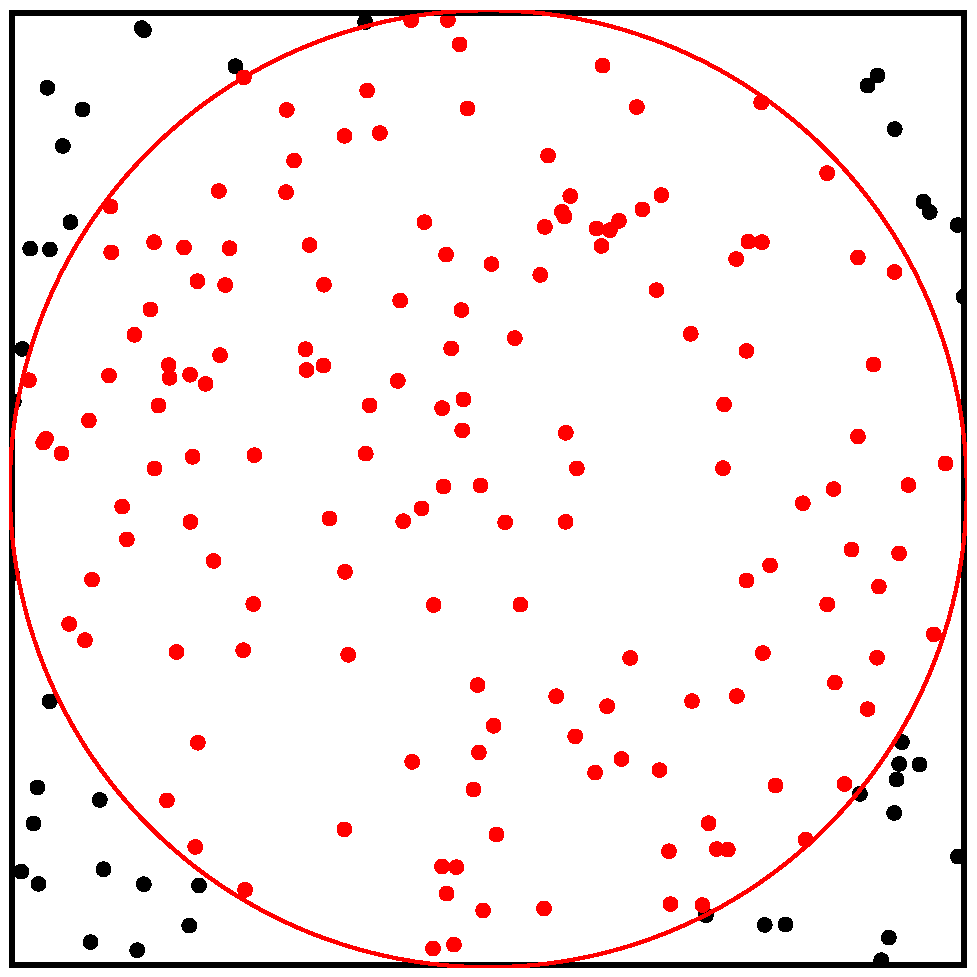
\includegraphics[width=0.35\textwidth]{picirc.pdf}
    \caption{Illustration of the rejection method for determining $\pi$ from the area of a circle inscribed within a square. The ratio of the area of the circle to the square is $\tfrac{\pi}{4}$. Thus the ratio of darts landing in the circle to those that land outside the circle is $\pi \approx \tfrac{4N_{inner}}{N_{total}}$, where $N_{total}$ is the total number of darts, and $N_{inner}$ is the total number of darts that land in the circle. Using 200 darts gave a value of $\pi \approx 3.12$}
    \label{fig:picircle}
\end{figure}


One common use of the Monte Carlo method, is to randomly sample from a spectrum.
To generate a random sample from a spectrum, first the \gls*{cdf} of the spectrum must be calculated.
This is done by first normalising the \gls*{pdf}, where the \gls*{pdf} in this case is the spectrum it self.
It is normalised such that the sum of the \gls*{pdf} is unity.
The \gls*{cdf} is then just the cumulative sum of the \gls*{pdf}.
Then using the above method as described above, a random number is drawn, $\xi$, and the bracketing values in the \gls*{cdf} are found.
We then interpolate to get the x and y values corresponding to $\xi$.
\Cref{fig:solar} shows the result of this process for 100 random samples.

\begin{figure}[!htbp]
    \centering
    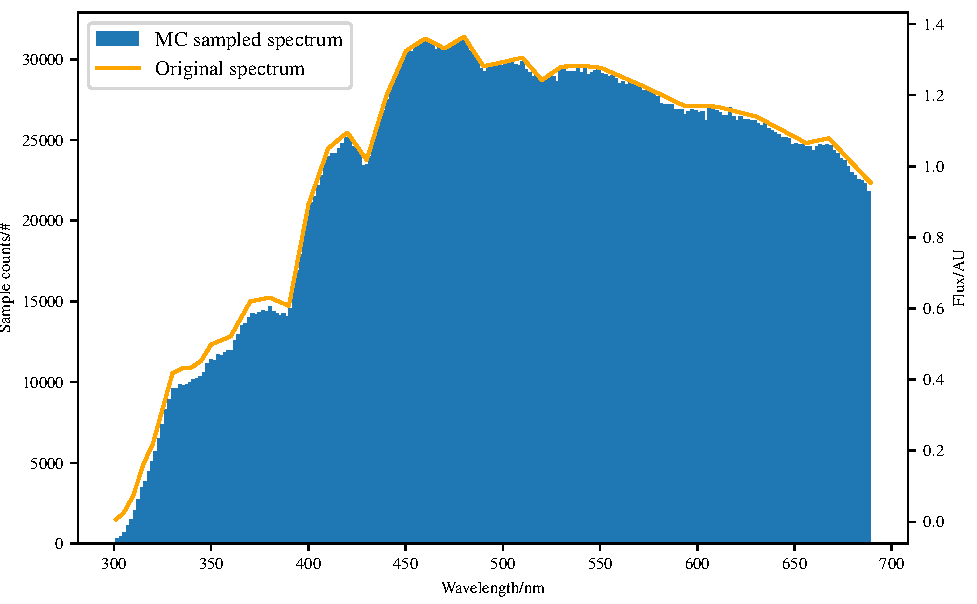
\includegraphics[width=0.75\textwidth]{solar-sample.pdf}
    \caption{Example of randomly sampling from a spectrum. Figure shows 100 random samples drawn to recreate a solar spectrum.}
    \label{fig:solar}
\end{figure}

The Monte Carlo method is used in various different disciplines. Ranging from use in the financial sector to analyse investments and stocks by simulating the sources of uncertainty which affect their values~\cite{jackel2002monte,finaceprrof}, use in statistical analysis~\cite{wall2012practical}, and in modern computer generated images (see \cref{fig:ray-trace})~\cite{Kajiyarendering,Cookraytracing}. It is also widely used in astronomy~\cite{robitaille2011hyperion,harries2014torus} and medicine~\cite{valentine2011monte,campbell2015monte}, to simulate the propagation of radiation through scattering (turbid) media. This technique, \gls*{mcrt}, is what makes up the bulk of this thesis and is described in depth in the following sections.

\begin{figure}[!htb]
\centering
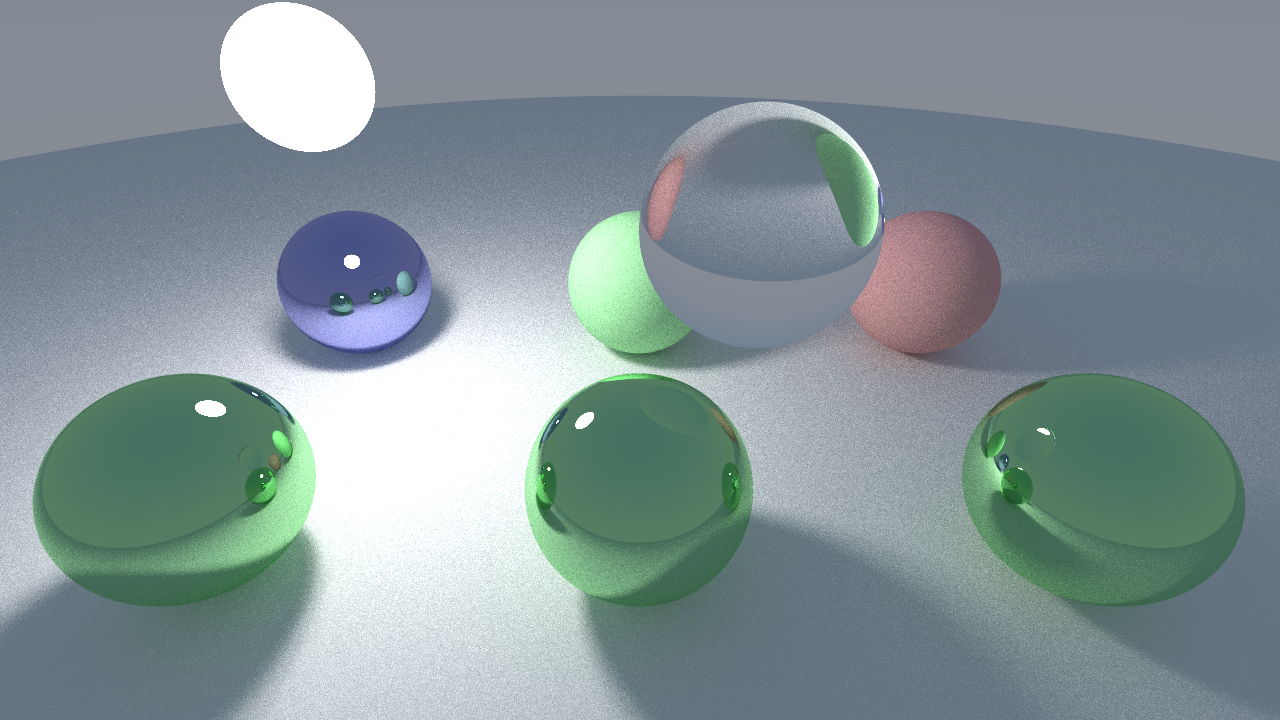
\includegraphics[width=.75\textwidth]{ray-tracing.png}
\caption{Computer generated imagery using ray tracing. The Monte Carlo method is used to ``compute radiance along ray paths between lights and the camera'', to generate CGI images~\cite{pharr2016physically}.}
\label{fig:ray-trace}
\end{figure}


\section{Synopsis and Thesis Objectives}
%sign post chapters

Chapter two details the Monte Carlo radiation transport method that is used for the bulk of this thesis.
Presented in this chapter are details of the algorithm and various code details that underpin the whole thesis.
Details of speed up techniques such as parallelisation are also presented.
Finally the code is validated against other results.\\


Chapter three details the tissue ablation model.
Discussion of the individual components of the model, alongside validation of the model against theoretical and experimental evidence is presented.\\


Chapter four presents an adaptation to the regular Monte Carlo model so that it can model wave like properties of photons including diffraction and interference.
The new algorithm is validated against several theoretical expressions and experimental data.
Finally the algorithm is used to compare Bessel beams and Gaussian beam in highly turbid media, to determine which beam preforms better.\\


Chapter five details the modelling of a novel biomarker for cardiovascular disease, autofluorescence.
The theoretical groundwork for the biomarker is outlaid, along with discussion of how Monte Carlo radiation transport can model fluorescence.
Presented alongside this is ameombaMCRT, a Monte Carlo radiation transfer simplex algorithm used to determine concentrations of fluorophores in different layers of tissue for a given spectrum.\\


Finally chapter six concludes this thesis and presents possible future avenues of research that could be undertaken.